\documentclass[11pt]{aghdpl}
% \documentclass[en,11pt]{aghdpl}  % praca w języku angielskim

% Lista wszystkich języków stanowiących języki pozycji bibliograficznych użytych w pracy.
% (Zgodnie z zasadami tworzenia bibliografii każda pozycja powinna zostać utworzona zgodnie z zasadami języka, w którym dana publikacja została napisana.)
\usepackage[english,polish]{babel}

% Użyj polskiego łamania wyrazów (zamiast domyślnego angielskiego).
\usepackage{polski}

\usepackage[utf8]{inputenc}

% dodatkowe pakiety

\usepackage{mathtools}
\usepackage{amsfonts}
\usepackage{amsmath}
\usepackage{amsthm}

% --- < bibliografia > ---

\usepackage[
style=numeric,
sorting=none,
%
% Zastosuj styl wpisu bibliograficznego właściwy językowi publikacji.
language=autobib,
autolang=other,
% Zapisuj datę dostępu do strony WWW w formacie RRRR-MM-DD.
urldate=iso8601,
% Nie dodawaj numerów stron, na których występuje cytowanie.
backref=false,
% Podawaj ISBN.
isbn=true,
% Nie podawaj URL-i, o ile nie jest to konieczne.
url=false,
%
% Ustawienia związane z polskimi normami dla bibliografii.
maxbibnames=3,
]{biblatex}

\usepackage{csquotes}
% Ponieważ `csquotes` nie posiada polskiego stylu, można skorzystać z mocno zbliżonego stylu chorwackiego.
\DeclareQuoteAlias{croatian}{polish}

\addbibresource{bibliografia.bib}

% Nie wyświetlaj wybranych pól.
%\AtEveryBibitem{\clearfield{note}}
% new macro - quotes

\newcommand{\quotes}[1]{``#1''}

% ------------------------
% --- < listingi > ---

% Użyj czcionki kroju Courier.
\usepackage{courier}

\usepackage{listings}
\lstloadlanguages{TeX}

\lstset{
	literate={ą}{{\k{a}}}1
           {ć}{{\'c}}1
           {ę}{{\k{e}}}1
           {ó}{{\'o}}1
           {ń}{{\'n}}1
           {ł}{{\l{}}}1
           {ś}{{\'s}}1
           {ź}{{\'z}}1
           {ż}{{\.z}}1
           {Ą}{{\k{A}}}1
           {Ć}{{\'C}}1
           {Ę}{{\k{E}}}1
           {Ó}{{\'O}}1
           {Ń}{{\'N}}1
           {Ł}{{\L{}}}1
           {Ś}{{\'S}}1
           {Ź}{{\'Z}}1
           {Ż}{{\.Z}}1,
	basicstyle=\footnotesize\ttfamily,
}

% ------------------------

\AtBeginDocument{
	\renewcommand{\tablename}{Tabela}
	\renewcommand{\figurename}{Rys.}
}

% ------------------------
% --- < tabele > ---

\usepackage{array}
\usepackage{tabularx}
\usepackage{multirow}
\usepackage{booktabs}
\usepackage{makecell}
\usepackage[flushleft]{threeparttable}

% defines the X column to use m (\parbox[c]) instead of p (`parbox[t]`)
\newcolumntype{C}[1]{>{\hsize=#1\hsize\centering\arraybackslash}X}


%---------------------------------------------------------------------------

\author{Piotr Konsek i Sebastian Batko}
\shortauthor{P. Konsek, S. Batko}

%\titlePL{Przygotowanie bardzo długiej i pasjonującej pracy dyplomowej w~systemie~\LaTeX}
%\titleEN{Preparation of a very long and fascinating bachelor or master thesis in \LaTeX}

\titlePL{Zastosowanie oprogramowania W3AF w testowanie aplikacji Moodle}
\titleEN{}

%\shorttitlePL{Przygotowanie pracy dyplomowej w~systemie \LaTeX} % skrócona wersja tytułu jeśli jest bardzo długi
%\shorttitleEN{Preparation of a long and fascinating thesis in \LaTeX}

\thesistype{}

\supervisor{}

\degreeprogramme{Informatyka}

\date{2016}

\department{Katedra Informatyki Stosowanej}

\faculty{Wydział Elektrotechniki, Automatyki,\protect\\[-1mm] Informatyki i Inżynierii Biomedycznej}

% TODO:
\acknowledgements{}


\setlength{\cftsecnumwidth}{10mm}

%---------------------------------------------------------------------------
\setcounter{secnumdepth}{4}

\begin{document}

\titlepages

% Ponowne zdefiniowanie stylu `plain`, aby usunąć numer strony z pierwszej strony spisu treści i poszczególnych rozdziałów.
\fancypagestyle{plain}
{
	% Usuń nagłówek i stopkę
	\fancyhf{}
	% Usuń linie.
	\renewcommand{\headrulewidth}{0pt}
	\renewcommand{\footrulewidth}{0pt}
}

\setcounter{tocdepth}{2}
\tableofcontents
\clearpage

\chapter{Wprowadzenie}
\label{cha:wprowadzenie}

Przedstawiony raport ma na celu przetestowania aplikacji Moodle, wykorzystując do tego celu oprogramowanie do testowania W3AF.

%---------------------------------------------------------------------------

\section{Zawartość raportu}
\label{sec:zawartoscPracy}
Struktura raportu jest następująca: 
\begin{itemize}
\item W pierwszym rozdziale opisany został program W3AF, jego konfiguracja oraz użyte pluginy. 
\item W rozdziale drugim omówiona została testowana aplikacja 
\item W rozdziale trzecim prezentujemy testy jakie przeprowadziliśmy na wybranej przez nas aplikacji.
\item W rozdziale czwartym zawarto wnioski 
\end{itemize}

%---------------------------------------------------------------------------

\section{W3AF}
W3AF (Web application attack and audit framework) to aplikacja open-source służąca do testowania bezpieczeństwa aplikacji internetowych Projekt zapewnia skaner podatności oraz narzędzia służące do wydobywania informacji z aplikacji internetowych. Dostarcza niezbędnych informacji o podatnościach na ataki dla wykonania testów penetracyjnych. Aplikacja dostarcza interfejs graficzny do wykonywania testów. Dostępny jest również interfejst tekstowy z linii komend.
\\
W3AF jest podzielony na dwie główne części, rdzeń oraz pluginy. Rdzeń koordynuje prace wszystkich procesów oraz dostarcza featury dostępne dla pluginów, które znajdują podatności oraz wykorzystują je. Pluginy są połączone ze sobą oraz dzielą się informacjami, używając do tego wspólnej bazy wiedzy. Pluginy mogą być podzielone na:
\begin{itemize}
\item Discovery
\item Audit
\item Grep
\item Attack
\item Output
\item Evasion
\item Bruteforce
\end{itemize}

\section{Użyte pluginy}

Do przetestowania aplikacji użyliśmy profilu OWASP\_TOP10, który bada aplikację pod kątem podatności na 10 najczęściej występujacych zagrożeń. Pluginy, które są wykorzystane to:
\begin{itemize}
\item csrf
\item htaccess\_methods
\item webspider
\item blind\_sqli
\item sqli
\item xss
\item buffer\_overflow
\end{itemize}

\section{Konfiguracja}

Niestety na systemie operacyjnym OSX nie jest możliwa praca z W3AF w trybie graficznym. Powodem tego jest występowanie błędu podczas uruchomienia. Spowodowane jest to bugiem w jednej z bibliotek pythona używanych do grafiki. Cała konfiguracja została zatem wykonana za pomocą linii komend. Aby uruchomić W3AF w linii komend, należy uruchomić skrypt a3wf\_console. Po uruchomieniu konsoli i wypisaniu prompta można przystąpić do konfiguracji frameworku. Z poziomu lini komend możemy dowolnie konfigurować działanie programu. Możemy wybrać, które pluginy będą używane, możemy, a nawet musimy skonfigurować cel naszych ataków w opcji target.
\noindent
\begin{minipage}{\linewidth}
\makebox[\linewidth]{
  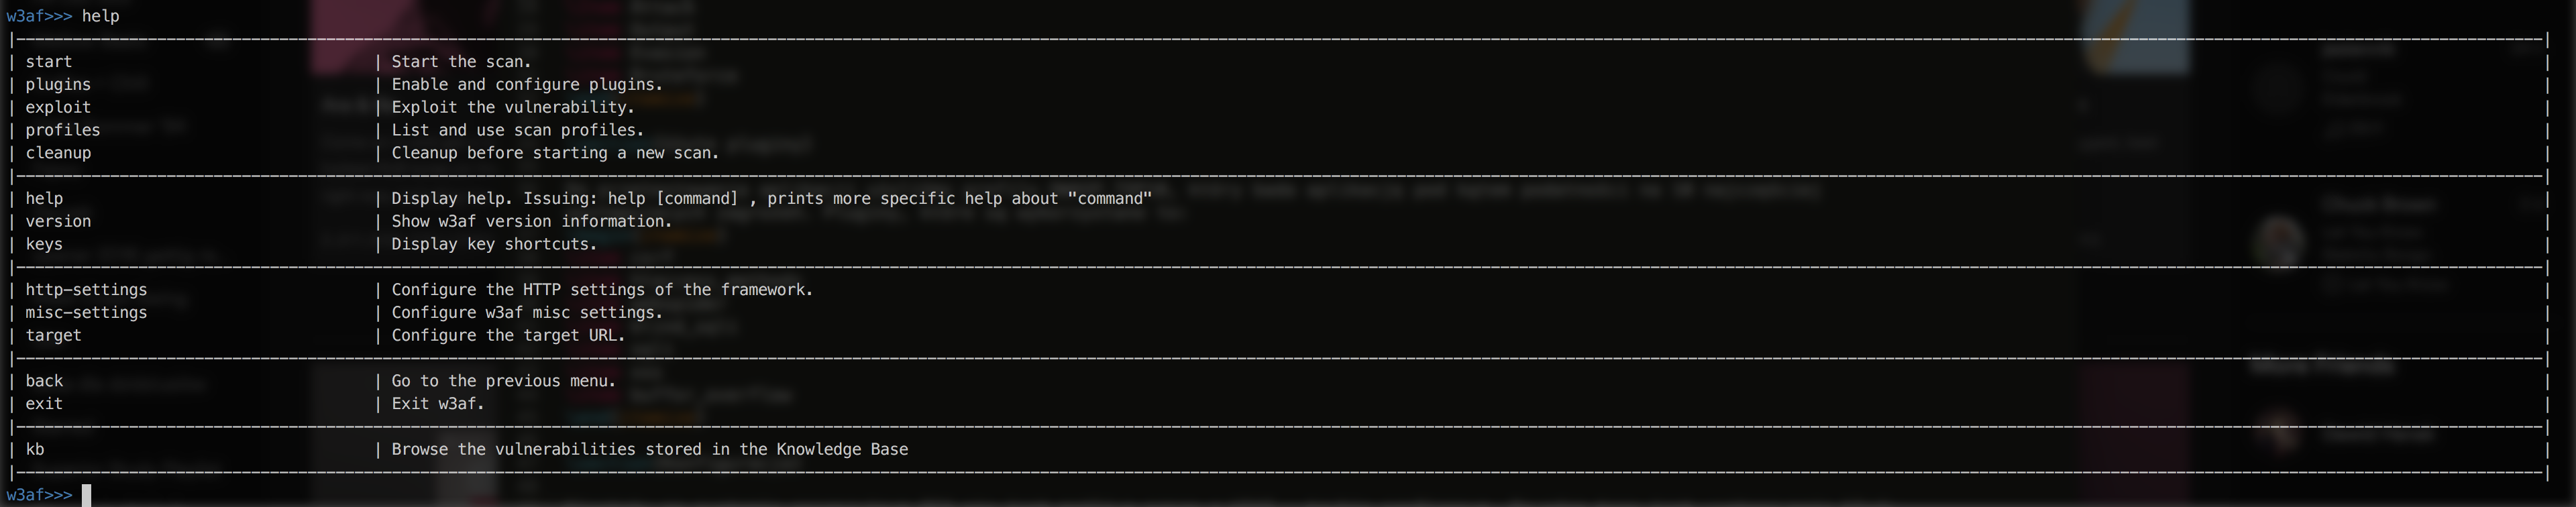
\includegraphics[keepaspectratio=true,scale=0.2]{pictures/options.png}}
\captionof{figure}{Opcje W3AF do wyboru}\label{erd}
\end{minipage}

\noindent
\begin{minipage}{\linewidth}
\makebox[\linewidth]{
  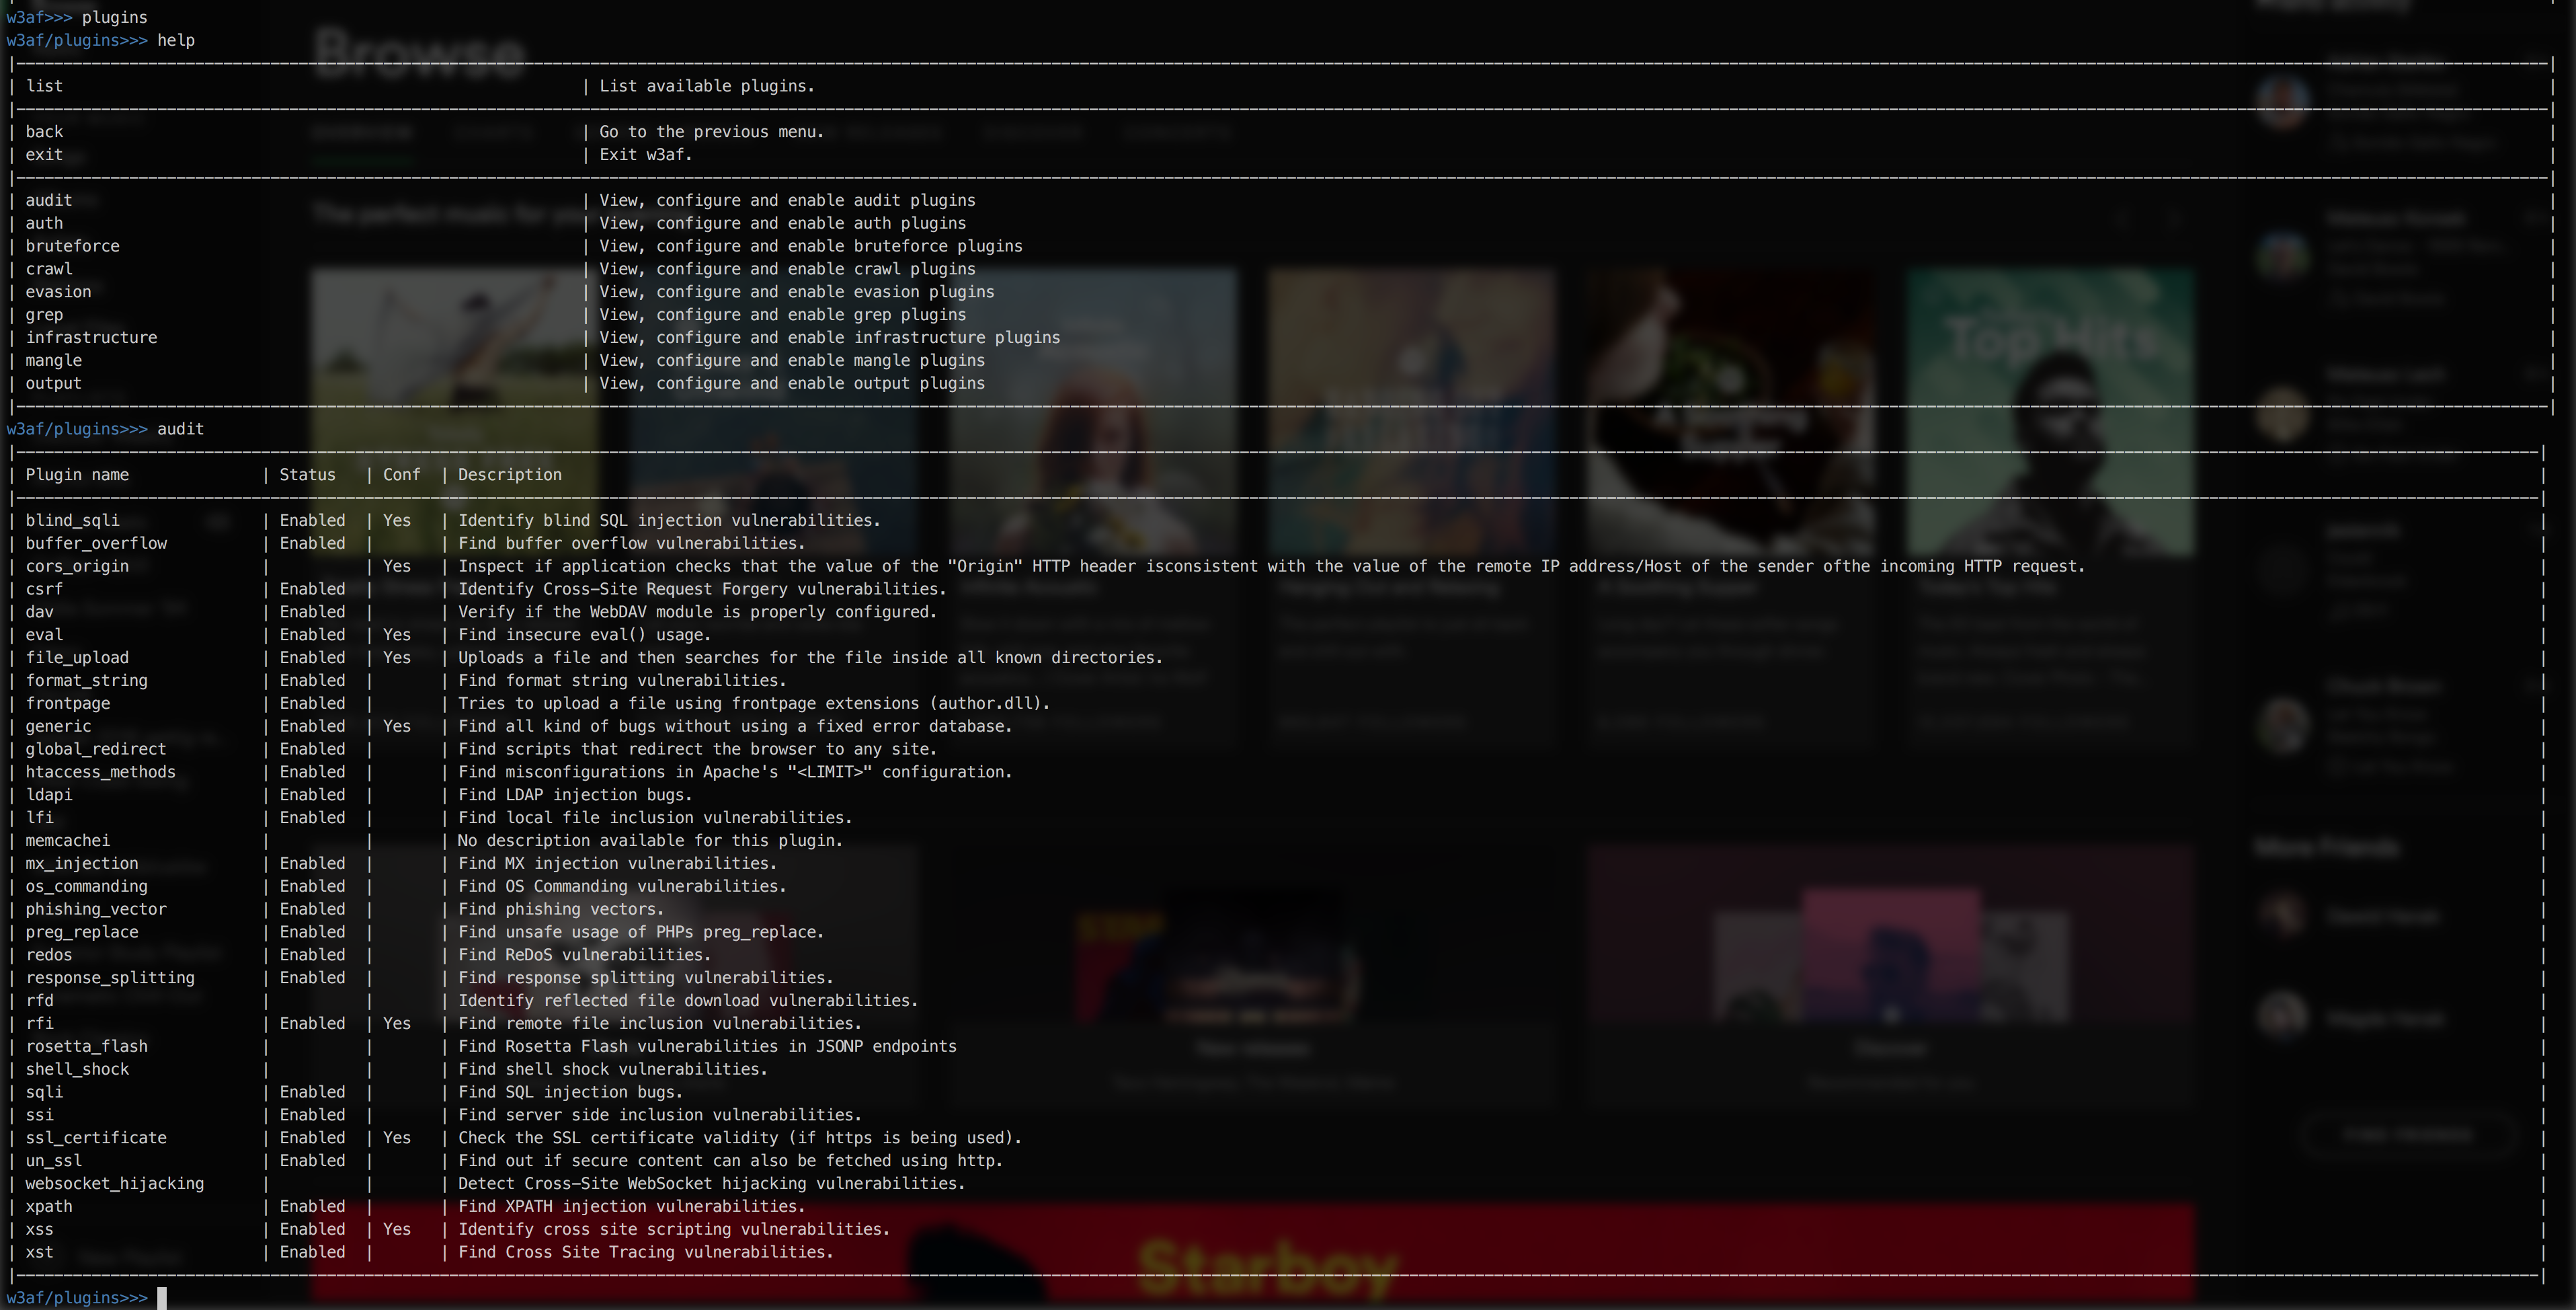
\includegraphics[keepaspectratio=true,scale=0.2]{pictures/plugins.png}}
\captionof{figure}{Różnorodność pluginów do wyboru}\label{erd}
\end{minipage}

\noindent
\begin{minipage}{\linewidth}
\makebox[\linewidth]{
  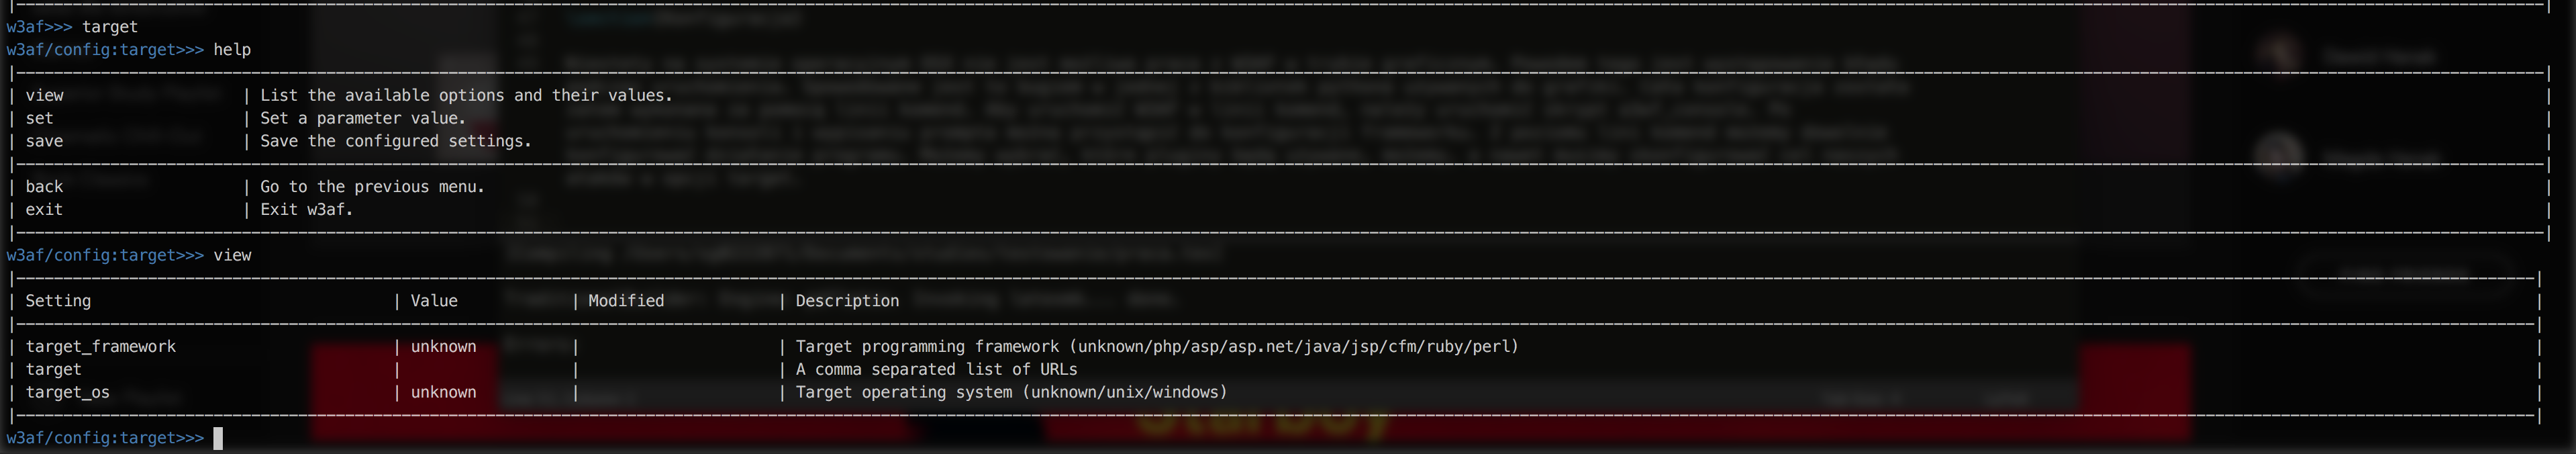
\includegraphics[keepaspectratio=true,scale=0.2]{pictures/target.png}}
\captionof{figure}{Konfiguracja celu ataków}\label{erd}
\end{minipage}

Ostatecznie główne testy przeprowadziliśmy wykorzystując tryb graficzny w3af na systemie Windows. W celu rozpoczęcia pracy należało ustawić URL docelowo testowanej aplikacji wraz z informacją na jakim systemie operacyjnym zostaną wykonane testy, a także technologię w jakiej napisany został testowany kod. Ustawienie tych elementów przedstawia poniższy zrzut:

\noindent
\begin{minipage}{\linewidth}
\makebox[\linewidth]{
  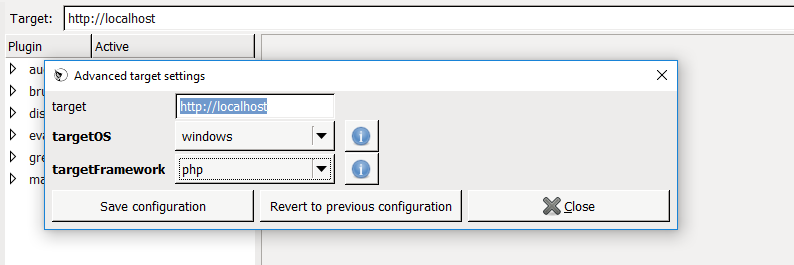
\includegraphics[keepaspectratio=true,scale=0.7]{pictures/w3afconf.png}}
\captionof{figure}{Konfiguracja w3af}\label{erd}
\end{minipage}
\end{enumerate}

W3af oferuje nam szereg różnego rodzaju testów wraz z gotowymi profilami do wyboru, które definiują określony sposób testowania aplikacji. Ten wachlarz możliwości widzimy na zrzucie:

\noindent
\begin{minipage}{\linewidth}
\makebox[\linewidth]{
  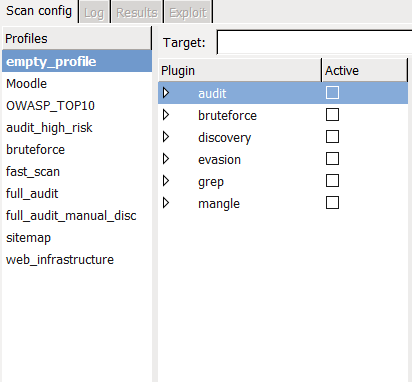
\includegraphics[keepaspectratio=true,scale=0.7]{pictures/w3aftests.png}}
\captionof{figure}{Profile oraz dostępne pluginy}\label{erd}
\end{minipage}
\end{enumerate}






\chapter{Moodle}
\label{cha:moodle}

Moodle to darmowy open-sourcowy program służący do zarządzania kursami uczelnialnymi. System jest napisany w PHP i dytstrybuowany pod licencją GNU. Stworzony z pedagogicznych pobudek, Moodle jest używany do różnorakiej nauki, zdalnej edukacji. Wykorzystując dostosowywalne zarządzanie opcjami, moodle jest używany do tworzenia prywatnych stron oferujących kursy internetowe dla trenerów oraz nauczycieli. Moodle ( akronim od Modular Object-Oriented Dynamic Learing Environment) pozwala na rozszerzanie i dopasowywania środowiska, wykorzystując szeroko dostępne w społeczności pluginy.

Struktura Moodle jest klasyczna dla portalu wymagającego posiadania kont. W Moodle każdy użytkownik posiada osobne konto, do którego przypisana jest jakaś rola. Rolą może być np. administrator, prowadzący kurs albo uczestnik. Żeby stworzyć konto należy się zarejestrować. Moodle jest napisany w całości w PHP, wykorzystuje serwer Apache oraz bazę danych PostgreSQL.

\chapter{Testy}
\label{cha:testy}

Poniżej prezentujemy testy jakie przeprowadzliśmy wraz z ich krótkim opisem oraz niezbędnymi zmianami w kodzie oraz komentarzem odnoszącym się do rezultatów otrzymywanych z w3af.

\section{Click-Jacking}
\begin{enumerate}
\item Opis podatności\\
CLick-Jacking to złośliwa technika nakłaniające użytkowników do klikania w inne rzeczy niż oni sami myślą, że klikają.
Może dojść do potencjalnego ujawnienia poufnych inforamcji lub przejęcia kontroli nad ich komputerem, po kliknięciu na pozornie niewinną stronę. Click-jacking przybiera też formę wbudowanego kodu lub skryptu, który może został wywołany bez wiedzy użytkownika.
\item Zmiany w kodzie\\
Nie były wymagane w przypadku tej podatności.
\item Komentarz\\
W3AF podczas pierwszego uruchomienia, bez zmian w kodzie, wykrył podatność aplikacji Moodle na brak zabezpieczeń przed atakami click-jacking. 
\end{enumerate}

\noindent
\begin{minipage}{\linewidth}
\makebox[\linewidth]{
  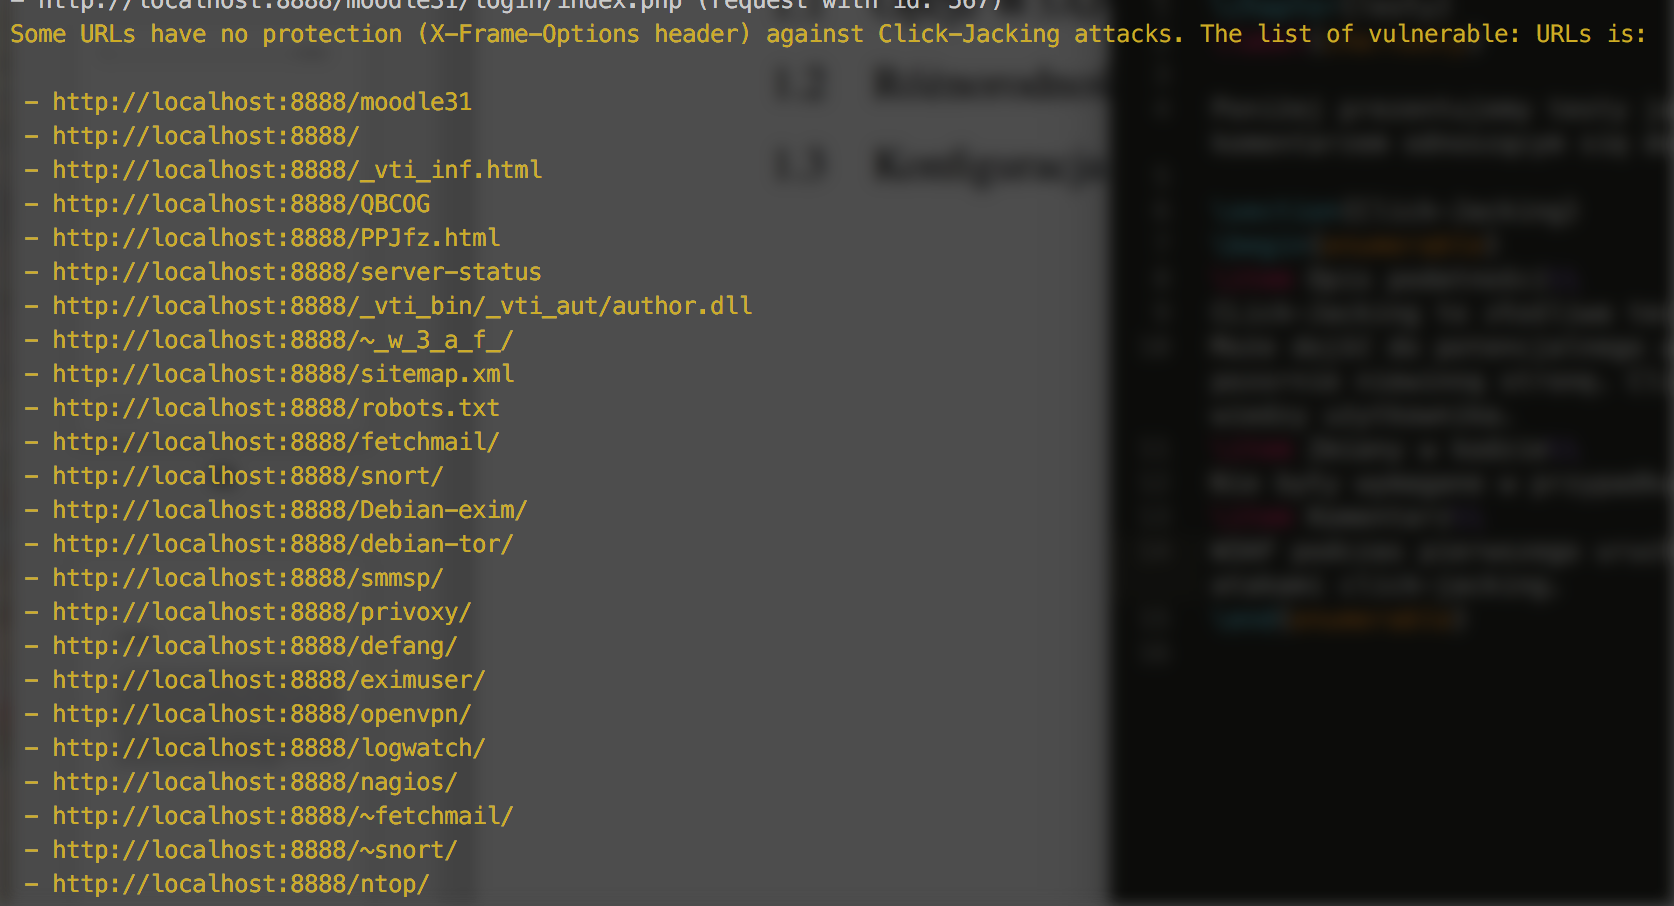
\includegraphics[keepaspectratio=true,scale=0.5]{pictures/clickjacking.png}}
\captionof{figure}{Wyniki W3AF dotyczące clickjackingu}\label{erd}
\end{minipage}

%--------------------------------------

\section{CSRF}
\begin{enumerate}
\item Opis podatności\\
CSRF - metoda ataku na serwis internetowy, która często (m.in. na skutek jednoczesnego wykorzystania) mylona jest z cross-site scripting (XSS) bądź jest uznawana za jej podzbiór. Ofiarami CSRF stają się użytkownicy nieświadomie przesyłający do serwera żądania spreparowane przez osoby o wrogich zamiarach. W przeciwieństwie do XSS, ataki te nie są wymierzone w strony internetowe i nie muszą powodować zmiany ich treści. Celem crackera jest wykorzystanie uprawnień ofiary do wykonania operacji w przeciwnym razie wymagających jej zgody. Błąd typu CSRF dotyczy również serwerów FTP. 
\item Zmiany w kodzie\\
Nie były wymagane w przypadku tej podatności.
\item Komentarz\\
W3AF znalazł podatność na CSRF podczas pierwszego uruchomienia testów:
\noindent
\begin{minipage}{\linewidth}
\makebox[\linewidth]{
  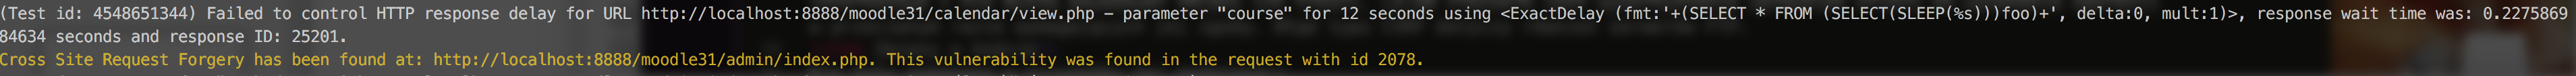
\includegraphics[keepaspectratio=true,scale=0.3]{pictures/csrf.png}}
\captionof{figure}{Wyniki W3AF dotyczące cross site request forgery}\label{erd}
\end{minipage}
\end{enumerate}


%--------------------------------------

\section{SQL injection}
\begin{enumerate}
\item Opis podatności\\
 metoda ataku komputerowego wykorzystująca lukę w zabezpieczeniach aplikacji polegającą na nieodpowiednim filtrowaniu lub niedostatecznym typowaniu danych użytkownika, które to dane są później wykorzystywane przy wykonaniu zapytań (SQL) do bazy danych. Podatne są na nią wszystkie systemy przyjmujące dane od użytkownika i dynamicznie generujące zapytania do bazy danych.
\item Zmiany w kodzie\\
Nie były wymagane w przypadku tej podatności.
\item Komentarz\\
W3AF, a konkretnie plugin blind\_sqli znalazł podatność na CSRF podczas pierwszego uruchomienia testów. Podatne na atak SQL injection są miejsca wpisywania loginu i hasła przez użytkownika.
\noindent
\begin{minipage}{\linewidth}
\makebox[\linewidth]{
  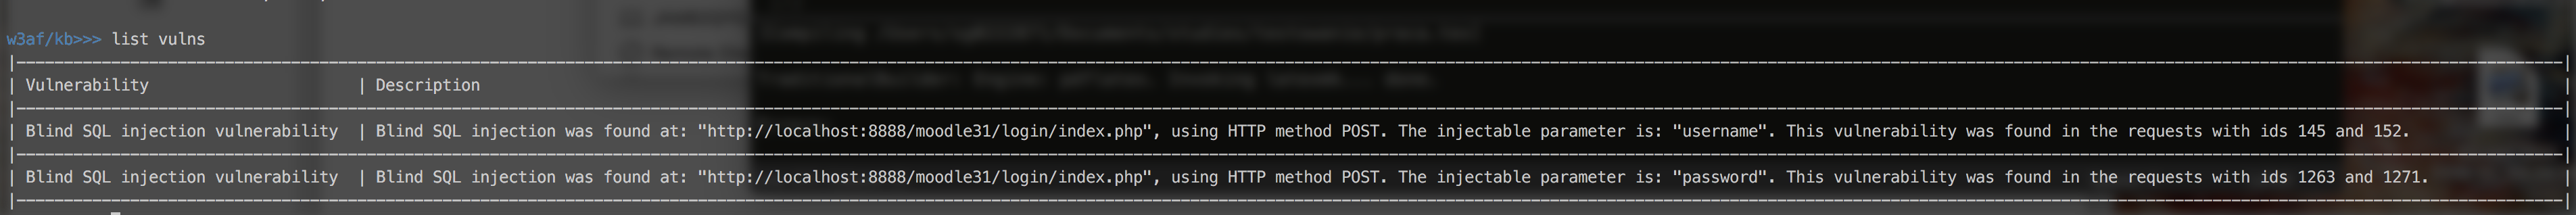
\includegraphics[keepaspectratio=true,scale=0.3]{pictures/sqli.png}}
\captionof{figure}{Wyniki W3AF z bazy wiedzy na temat sql injection}\label{erd}
\end{minipage}
\end{enumerate}

% \chapter{Wnioski}

Narzędzie jest bardzo pożytecznym oprogramowaniem. Dla niektórych może się to wydawać trochę dziwne, biorąc pod uwagę fakt, że program jest udostępniany na zasadach licencji open-source. W efekcie prac nad tą aplikacją, powstało oprogramowanie słuażce zabezpieczaniu aplikacji webowych poprzez znajdowanie w nich wszelkiego rodzaju luk bezpieczeństwa.\\

Zaletą narzędzia jest z pewnością mnogich dostępnych pluginów oraz udostępnianych przez nie testów, które można przeprowadzić na dowolnej aplikacji webowej Użytkownik otrzymuje około setki pluginów, które można ze sobą łączyć w dowolny sposób. Każde, dowolne ustawienie konfiguracji można zapisać w postaci profilów. Użytkownik oprogramowania W3AF dostaje out-of-the-box kilka prekonfigurowanych profili z których może korzystać. Wśród tych profili znajduje się między innym OWASP\_TOP10 zawierajcy konfigurację pozwalająca na przetestowanie aplikacji pod kątem 10 najczęściej występujących luk w zabezpieczeniu aplikacji. Lista ta została stworzona przez grupę ekspertów na podstawie badań i ankiet przeprowadzonych wśród topowych dostawców treści internetowych. \\

Dodatkową zaletą aplikacji jest łatwość, z jaką możemy przeglądać zgromadzoną przez program wiedzy w trakcie działania. Minusem jest niestety niska zdolnośc aplikacji do agregacji (łączenia) ze sobą różnych rezultatów. Na szczęście program umożliwia eksport wyników do pliku tekstowego. Do największych wad aplikacji należy jej stabilność oraz brak możliwościu uruchomienia trybu graficznego na sytemie operacyjnym OSX.\\

Naszym zdaniem, używana przez nas aplikacja jest ciekawym narzędziem dostarczającym wiedzę o podstawowych lukach bezpieczeństwa w aplikacji. W3AF może nie jest w stanie ostrzec nas przed bardziej wyrafinowanymi próbami dostępu, lecz jest doskonałym narzędziem wskazującym na podstawowe luki bezpieczeństwa, takiej jak XSS lub clickjacking. Z pewnością, gdyby w3af było rozwijane przez większą liczbę programistów, rezultaty oraz stabilność aplikacji uległaby poprawie.\\

Podsumowując, W3AF jest bardzo ciekawym produktem środowiska open-sourcowego. Nie należy z całkowitą ufnością wierzyć wynikom dostarczanych przez programowanie. Rezultaty jednak mogą być dosyć dobrą wskazówką, gdzie należy szukać podatności aplikacji na ataki.
% \chapter{Podręcznik użytkownika}
\label{cha:podrecznik uzytkownika}

Poniżej opisane są kroki umożliwiające szybkie i bezproblemowe uruchomienie stworzonej aplikacji w środowisku lokalnym. 

%------------------------------------------------------------------------------------------------

\section{Wymagania dotyczące środowiska pracy}
Aby korzystać z zaimplementowanej aplikacji niezbędne jest:
\begin{itemize}
\item środowisko z systemem operacyjnym OSX lub Linux
\item środowisko z zainstalowanym interpreterem języka Ruby w wersji 2.1.5
\item dostęp do internetu w celu pobrania zależności projektu.
\item przeglądarka internetowa z włączoną obsługą języka JavaScript.
\end{itemize}
Jeżeli środowisko jest wyposażone w powyższe elementy, należy pobrać wszystkie zależności za pomocą polecenia \textit{bundle install}, oraz uruchomić serwer poleceniem \textit{bundle exec rail s}. Aplikacja zostanie uruchomiona na serwerze lokalnym w domyślnej konfiguracji. Aby otworzyć aplikację w przeglądarce, należy wpisać adres \textit{localhost:3000}.

%------------------------------------------------------------------------------------------------

\newpage

\section{Rejestracja}
\label{sec:rejestracja}
Aby się zarejestrować, należy kliknąć lewym przyciskiem myszy na przycisku \quotes{Registration} znajdującym się w prawym górnym rogu aplikacji. Po kliknięciu na ekranie powinno pojawić się dodatkowe okno z formularzem rejestracji. Po poprawnym wypełnieniu formularza rejstracji, użytkownik powinien od razu zostać zalogowany do systemu.\\
\\
\begin{minipage}{\linewidth}
\makebox[\linewidth]{
  \includegraphics[keepaspectratio=true,scale=0.8]{pictures/registration.png}}
\captionof{figure}{Rejestracja}\label{registration}
\end{minipage}\\

\newpage

%------------------------------------------------------------------------------------------------

\section{Logowanie}
\label{sec:logowanie}
Aby się zalogować, należy kliknąć lewym przyciskiem myszy na przycisku \quotes{Login} znajdującym się również w prawym górnym rogu formularza obok przycisku służącego do rejestracji. Po jego naciśnięciu, na ekranie powinno pojawić się dodatkowe okienko z formularzem logowania. Po poprawnym wypełnieniu formularza oraz autentykacji, użytkownik powinien zostać zalogowany do sytstemu. 
Po zalogowaniu użytkownika na pasku powinny pojawić się przycisku służące do dodania nowej oferty, edycji profilu użytkownika oraz wylogowania się.\\
\\

\begin{minipage}{\linewidth}
\makebox[\linewidth]{
  \includegraphics[keepaspectratio=true,scale=0.8]{pictures/login.png}}
\captionof{figure}{Logowanie}\label{login}
\end{minipage}\\

\newpage

%------------------------------------------------------------------------------------------------

\section{Dodanie oferty}
Aby dodać nową ofertę, należy kliknąć lewym przyciskiem myszy na przycisk opatrzony nazwą \quotes{Add offer}. Po kliknięciu powinien pojawić się okno z formularzem umożliwiającym wpisania danych.\\
\\
\begin{minipage}{\linewidth}
\makebox[\linewidth]{
  \includegraphics[keepaspectratio=true,scale=0.5]{pictures/add-offer1.png}}
\captionof{figure}{Dodawanie nowej oferty}\label{add-offer1}
\end{minipage}\\

\newpage

Po kliknięciu przycisku \quotes{Submit} i poprawnej walidacji, użytkownik zostaje przeniesiony do okna umożliwiającego dodawanie zdjęć. Po wybraniu zdjęcia należy kliknąć przycisk \quotes{Create Photo} aby wysłać zdjęcie na serwer. Po poprawnej operacji zapisu zdjęcia, powinno się ono pojawić na górze formularza. Mały przycisk w kształcie litery X przy zdjęciu służy do jego usuwania.\\
\\
\begin{minipage}{\linewidth}
\makebox[\linewidth]{
  \includegraphics[keepaspectratio=true,scale=0.6]{pictures/add-offer2.png}}
\captionof{figure}{Dodawanie zdjęć do oferty}\label{add-offer2}
\end{minipage}\\

\newpage

Po kliknięciu przycisku \quotes{Next} użytkownik zostaje przeniesiony do ostatniego etapu tworzenia nowego ogłoszenia, w którym musi określić precyzjną lokalizację oferty. Dokładną lokalizację użytkownik może wybrać poprzez kliknięcie na mapie. W ten sposób zostaje określona długość i szerokość geograficzna. Po wypełnieniu pozostałych pól formularza i kliknięciu przycisku \quotes{Submit}, oferta powinna pojawić się na głównej mapie.\\
\\
\begin{minipage}{\linewidth}
\makebox[\linewidth]{
  \includegraphics[keepaspectratio=true,scale=0.5]{pictures/add-offer3.png}}
\captionof{figure}{Określanie lokalizacji oferty}\label{add-offer3}
\end{minipage}\\

%------------------------------------------------------------------------------------------------

\section{Edycja oferty}
Jeżeli użytkownik naciśnie lewym klawiszem myszki na marker znajdujący się na głównej mapie, powinno się otworzyć okienko przedstawiające informacje o ofercie. Jeżeli dana oferta należy do użytkownika to oprócz informacji widocznych dla innych użytkowników, dostępny jest dla niego przycisk \quotes{Edit offer}, który przenosi użytkownika do formularza edycji oferty. \ref{delete-offer}\\
\\
\begin{minipage}{\linewidth}
\makebox[\linewidth]{
  \includegraphics[keepaspectratio=true,scale=0.5]{pictures/edit-offer.png}}
\captionof{figure}{Edytowanie oferty}\label{edit-offer}
\end{minipage}\\

%------------------------------------------------------------------------------------------------

\section{Usunięcie oferty}
Po otworzeniu okna edycji oferty, na dole strony widoczny jest przycisk służący do usuwania danej oferty. Usunięcie oferty wiąże się z usunięciem wszystkich zdjęć i lokalizacji dołączonych do oferty.\\
\\
\begin{minipage}{\linewidth}
\makebox[\linewidth]{
  \includegraphics[keepaspectratio=true,scale=0.5]{pictures/delete-offer.png}}
\captionof{figure}{Usuwanie oferty}\label{delete-offer}
\end{minipage}\\ 

%------------ FILTROWANIE WYNIKÓW ----------------

\section{Filtrowanie wyników}
Filtrowanie wyników jest opcją dostępną zarówno dla niezalogowanych jak i zalogowanych użytkowników. Filtry znajdują się po lewej stronie aplikacji na liście z możliwością chowania. Jedyną różnicą pomiędzy używaniem filtrów dla użytkowników, to możliwość zapisania filtrów przez zalogowanego użytkownika. Po kliknięciu myszką na mapę, pojawia się na niej znacznik w kształcie okręgu. Jest to znacznik środka obszaru zainteresowań użytkownika. Promień tego obszaru użytkownik może zmieniac za pomocą pierwszego suwaka na liście filtrów. Pozostałe filtry odnoszą się bezpośrednio do atrybutów oferty.\\
\\
\begin{minipage}{\linewidth}
\makebox[\linewidth]{
  \includegraphics[keepaspectratio=true,scale=0.4]{pictures/filters.png}}
\captionof{figure}{Filtrowanie ofert}\label{filters}
\end{minipage}\\ 

%------------  WATCHED OFFERS ----------------

\section{Dodanie oferty do obserwowanych}
Jeżeli użytkownik naciśnie lewym klawiszem myszki na marker znajdujący się na głównej mapie, powinno się pojawiić okienko przedstawiające ofertę. Jeżeli dana oferta nie należy do użytkownika wtedy nie zostanie wyświetlony przycisk służący do przejścia do edycji oferty. Pojawi się natomiast przycisk służący do dodania oferty do obserwowanych ofert. Po kliknięciu tego przycisku i dodaniu oferty do obserwowanych, zmieni się on w przycisk służący odwrotnej akcji, czyli usunięcia oferty z listy obserwowanych.\\
\\
\begin{minipage}{\linewidth}
\makebox[\linewidth]{
  \includegraphics[keepaspectratio=true,scale=0.5]{pictures/watch-offer.png}}
\captionof{figure}{Dodawanie ofert do obserwowanych}\label{watch-offer}
\end{minipage}\\ 

% \chapter{Testy systemu}
\label{cha;testySystemu}

Zostały przeprowadzone manualne testy aplikacyjne, które zweryfikowały czy powstała aplikacja spełnia postawione mu wymagania. Oprócz testów manualnych zostały wykonane również testy behawioralne napisane we frameworku RSpec. Testy behawioralne zostały napisane zgodnie z metodyką  TDD (Test Driven Development). Wymagania, które zostały przetestowane na działającym serwisie to:
\begin{itemize}
\item niezawodność,
\item intuicyjność interfejsu,
\item bezpieczeństwo danych,
\item odporność na nieautoryzowany dostęp do danych.
\end{itemize}
Oprócz sprawdzenia czy system spełnia postawione przed nim wymagania, przetestowane zostały również funkcjonalności wyspecyfikowane w rozdziale 2. \textit{Analiza wymagań}

\section{Scenariusze testowania}
Najważniejsze funkcjonalności systemu były przetestowane wzorując się na poniższych scenariuszach:
 \begin{enumerate}
 \item Rejestracja
 \begin{itemize}
 \item Warunki początkowe:
 \begin{itemize}
 \item W sesji przeglądarki nie znajduję się sesja należąca do żadnego użytkownika
 \end{itemize}
 \item Kroki testowe:
 \begin{enumerate}
 \item Naciśnięcie przycisku \textbf{Registration} - w odpowiedzi powinno pojawić się dodatkowe okno z formularzem rejestracji.
 \item Wprowadzenie niepoprawnych danych takich jak:
 \begin{itemize}
 \item Brak któregokolwiek z atrybutów formularza
 \item Niepoprawny adres mailowy
 \item Adres mailowy jest już wykorzystany
 \item Zbyt krótkie hasło
 \end{itemize}
 Spowoduje błąd walidacji formularza w skutek czego, użytkownik zostanie poinformowany o przyczynie niepowodzenia. Pola formularza oprócz hasła powinny pozostać niezmienione.
 \item Wprowadzenie poprawnych danych skutkuje utworzeniem profilu użytkowniku w aplikacji oraz automatycznym zalogowanie użytkownika do aplikacji.
 \end{enumerate}
 \end{itemize}

 \item Logowanie 
  \begin{itemize}
   \item Warunki początkowe:
    \begin{itemize}
     \item W sesji przeglądarki nie znajduje się sesja należąca do żadnego użytkownika
     \item Istnieje co najmniej jeden profil użytkownika
    \end{itemize}
   \item Kroki testowe:
    \begin{enumerate}
     \item Naciśnięcie przyscisku \textbf{Login} - w odpowiedzi powinno pojawić się dodatkowe okno z formularzem logowania
     \item Wprowadzenie niepoprawnych danych takich jak:
      \begin{itemize}
       \item Brak adresu mailowego lub hasła
       \item Adres mailowy niewystępujacy w bazie danych
       \item Hasło nie pasujące do podanego adresu mailowego
      \end{itemize}
      Spowoduje błąd walidacji formularza, w skutek czego, użytkownik zostanie poinformowany o przyczynie niepowodzenia. Pole adresu mailowego powinno zostać niezmienione.
     \item Wprowadzenie poprawnych danych skutkuje zalogowaniem użytkownika dla aplikacji oraz dodaniem do ciasteczek obiektu z informacją o sesji użytkownika.
    \end{enumerate}
  \end{itemize}

 \item Dodawanie oferty
  \begin{itemize}
   \item Warunki poczatkowe:
    \begin{itemize}
     \item Użytkownik jest zalogowany do systemu
    \end{itemize}
   \item Kroki testowe:
    \begin{enumerate}
     \item Naciśnięciu przycisku \textbf{Add offer} - w odpowiedzi powinno pojawić się dodatkowe okno z formularzem tworzenia nowej oferty
     \item Wprowadzenie nieporawnych danych spowoduje błąd walidacji oraz wyświetlenie odpowiednich komunikatów o przyczynie niepowodzenia walidacji
     \item Wprowadzenie poprawnych danych oraz naciśnięcie przycisku \textbf{Submit} powoduje przejście do następnego okna zawierającego formularz dodawania zdjęć.
     \item Wybranie przycisku dodawania zdjęcia powinno otworzyć okno z systemową przeglądarką plików.
     \item Naciśnięcie przycisku \textbf{Submit} spowoduje próbę zapisu zdjęcia - jeżeli format pliku nie należy do obsługiwanych przez aplikację, zdjęcie nie zostanie dodane. W przeciwnym wypadku zapis zdjęcia zakończy się powodzeniem oraz przejściem do formularza dodania lokalizacji.
     \item Wybranie przycisku \textbf{Create another} spowoduję zapisanie zdjęcia przy zachowaniu warunków podanych powyżej. Następnie wróci do formularza dodawnia zdjęcia, wyświetlając już dodane zdjęcia.
     \item W formularzu oferty należy zaznaczyć pozycję na mapie oraz podać dokładny adres w przeciwnym wypadku użytkownik powinien zostać poinformowany o przyczynach braku sukcesu po kliknięciu przycisku \textbf{Submit}
     \item Jeżeli wszystkie dane w formularzu lokalizacji są walidowalne, oferta powinna zostać utworzona. Na mapie powinien się natychmiast pojawić znacznik odpowiadający lokalizacji danej oferty.
    \end{enumerate}
  \end{itemize}

 \item Wyświetlanie oferty
  \begin{itemize}
   \item Warunki początkowe:
    \begin{itemize}
     \item W aplikacji istnieje co najmniej jedna oferta.
    \end{itemize}
   \item Kroki testowe:
    \begin{enumerate}
     \item Naciśnięcie znacznika na mapie reprezentującego ofertę
     \item Użytkownik powinien zaobserwować pojawienie się nowego okna wypełnionego danymi oferty
     \item Użytkownik do którego należy dane ogłoszenie powinien (będąc zalogowanym) widzieć opcję edycji ogłoszenia.
     \item Zalogowany użytkownik do którego nie należy dane ogłoszenie powinien mieć możliwość dodania oferty do obserwowanych ofert.
     \item Użytkownik zarejestrowany i niezarejestrowany powinien mieć możliwość zamknięcia oferty klikając na krzyżyk znajdujący się w prawym górnym rogu lub gdziekolwiek poza ofertą.
    \end{enumerate}
  \end{itemize} 

 \item Edycja oferty
  \begin{itemize}
   \item Warunki początkowe:
    \begin{itemize}
     \item Użytkownik jest zalogowany
     \item W aplikacji istnieje co najmniej jedna oferta przypisana dla zalogowanego użytkownika
    \end{itemize}
   \item Kroki testowe:
    \begin{enumerate}
     \item Naciśnięcie znacznika na mapie reprezentującego ofertę
     \item Użytkownik powinien zaobserwować pojawienie się nowego okna wypełnionego danymi oferty
     \item Użytkownik do którego należy dane ogłoszenie powinien (będąc zalogowanym) widzieć opcję edycji ogłoszenia. Po naciśnięciu tego przycisku powinno pojawić się okno z formularzem służącym do edytowania informacji o ofercie.
     \item Kliknięcie przycisku \textbf{Submit} w przypadku pozytywnej walidacji zapisuje zmiany i przenosi użytkownika do formularza edycji zdjęć. W przeciwnym wypadku użytkownik zostaje powiadomiony o przyczynie niepowodzenia walidacji.
     \item Użytkownik może dodać kolejne zdjęcia lub usunąć już istniejące za pomocą przycisku w kształcie litery \textbf{X}.
     \item Po skończeniu edycji użytkownik powinien zostać przeniesiony do formularza edycji lokalizacji.
     \item Po naciśnięciu przycisku \textbf{Submit} oferta powinna zostać zaktualizowana lub w przypadku niepoprawnej walidacji, powinnny zostać wyświetlone odpowiednie informacje o przyczynach niepowodzenia walidacji. W przypadku poprawnego zakończenia procesu walidacji oraz zapisywania formularz edycji powinien się  zamknąć, a znacznik oferty na mapie powinien udostępniać zakutalizowane dane.
    \end{enumerate}
  \end{itemize} 

 \item Zapisanie filtrów
  \begin{itemize}
   \item Warunki początkowe:
    \begin{itemize}
     \item Użytkownik jest zalogowany
     \item Istnieje co najmniej jedna oferta (warunek konieczny do zweryfikowania działania filtrów)
    \end{itemize}
   \item Kroki testowe:
    \begin{enumerate}
     \item Zalogowany użytkownik powinien widzieć na dole panelu z filtrami opcję zapisania filtrów. Po klinięciu przycisku użytkownik powinien zostać poinformowany o wyniku procesu zapisywania filtrów.
     \item Użytkownik po wylogowaniu i ponownym zalogowaniu do aplikacji powinien mieć filtry w takim samym stanie jak w momencie zapisu.
     \item Ponowne zapisanie filtrów powoduje nadpisanie poprzednich zapisanych fitrów.
     \item Po usunięciu zapisanych filtrów użytkownik powinien mieć filtry ustawione w pozycji domyślnej 
    \end{enumerate}
  \end{itemize}

 \item Zliczanie wyświetleń oferty
  \begin{itemize}
   \item Warunki początkowe:
    \begin{itemize}
     \item Istnieje co najmniej jedna oferta
    \end{itemize}
   \item Kroki testowe:
    \begin{enumerate}
     \item Należy otworzyć ofertę, zanotować aktualną liczbę wyświetleń, zamknąć ofertę.
     \item Po ponownym otwarciu oferty liczba wyświetleń powinna się zwiększyć o jeden (lub o co najmniej jeden w przypadku testowania aplikacji na środowisku produkcyjnym).
    \end{enumerate}
  \end{itemize}
\end{enumerate}

\section{Realizacja testów}
Relizacja testów jest oparta o framework RSpec, który został stworzony na potrzeby testowania kodu napisanego w języku Ruby. RSpec udostępnia mechanizmy ułatwiające proces testowania takie jak fabryki obiektów, fabryki losowych danych. Z czasem framework został dostosowany również do testowania frameworku Rails. Testy składają  się z testów:
\begin{itemize}
\item jednostkowych,
\item funkcjonalnych.
\end{itemize}
Testy jednostkowe służą do sprawdzania możliwie najmniejszych fragmentów kodu. Przykladem testu jednostkowego jest sprawdzenie czy metoda sprawdzająca przynależność oferty do użytkownika rzeczywiście działa zgodnie z założeniami w przypadku danych wejściowych dających poprawne i niepoprawne rezultaty. Funkcje są sprawdzane również pod kątem odporności na błędne dane wejściowe takie jak złe typy, brak wartości. W takich przypadkach funkcjonalność sprawdza, czy został wyrzucony wyjątek jeżeli tak została funkcja zaprojektowana, czy też wyjątek został poprawnie obsłużony wewnątrz funkcji. Testy jednostkowe są bardzo pożyteczne w trakcie tworzenia oprogramowania, gdyż od samego początku umożliwiają wykrycie niepożądanych zachowań\\
\\
Testy funkcjonalne służą do sprawdzenie poprawości całych funkcjonalności takich jak logowanie czy rejestracja. Testowanie odbywa się na podstawie wymagań jakie dana funkcjonalność powinna spełniać. Testy te, są szczególnie przydatne przy procesie rozwijania oprogramowania, dodawnia nowych funkcjonalności. Wykonując te testy można się upewnić, że żadna funkcjonalność nie została naruszona podczas tworzenia innych fragmentów kodu.

\section{Analiza wyników testów}
Testy zostały przeprowadzone tylko dla części back-endowej z uwagi na brak możliwości przetestowania części front-endowej za pomocą frameworka RSpec. Zakładając, że wszystkie napisane testy w poprawny sposób testują funkcjonalności, aplikacja została przetestowana niemalże całkowicie. Wszystkie napisane testy dają wynik pozytywny przy jednoczesnym braku niedeterminizmu.

% \chapter{Podsumowanie}
\label{cha:podsumowanie}

Poniższy rozdział zawiera podsumowanie pracy nad projektem oraz implementacją. Zostały tu zawarte wnioski wyciagnięte podczas trwania prac nad aplikacją oraz przedstawione są możliwości dalszego jej rozwoju.

\section{Wnioski}
W ramach tej pracy inżynierskiej została przygotowana aplikacja służąca do zamieszczania i łatwego wyszukiwania ofert nieruchomości. Wykonana aplikacja jest wynikiem wielu procesów, które musiały zostać zrealizowane. W pierwszej kolejności konieczne było zaznajomienie się z zagadnieniem oraz przeglądnięcie podobnych serwisów. Następnie, niezbędnym elementem była analiza wymagań, która została przeprowadzona opierając się na doświadczeniach wyniesionych z poprzedniego etapu oraz na własnej kreatywności. W kolejnych etapach pracy został zrealizowany konkretny projekt systemu, właczając w to opis funkcjonalności, konkretnych obiektów. Ważnym elementem tworzenia aplikacji były testy przeprowadzane metodą TDD. Pozwoliło to na uniknięcie błędów, które mogłyby być, trudne do naprawienia przy implementacji innych funkcjonalności. Sumą  tych wszystkich składników jest kompletna i działająca aplikacja realizująca wyspecyfikowane zadania.\\
Problemy, które zostały napotkane w trakcie pisania pracy to:
\begin{itemize}
\item Zabezpieczenie treści przed niepowołanym odczytem - bezpieczeństwo aplikacji zostało opisane w sekcji \quotes{Autoryzacja i autentykacja} \ref{sec:autoryzacjaAutentykacja}
\item Wydajne filtrowanie logicznych atrybutów ofert - zostało to rozwiązane za pomocą sprawdzania zawierania się zbiorów zmiennych pochodzących z filtrów oraz z oferty.
\end{itemize}

\section{Możliwość rozwoju}
Aplikacja została napisana w sposób, który umożliwa jej dalsze rozszerzanie. Jedną z możliwości rozwoju, która bardzo znacząco poprawiłaby jakość serwisu, byłaby możliwość przeszukiwania ofert mieszkań w sieci internetowej i zapisywanie ich do aplikacji. Jest to zadanie jednakże trudne, gdyż wiele ofert w sieci nie posiada zbyt szczegółowych informacji oraz jest zapisana w wielu różnych formatach oraz konwencjach. Kolejnym naturalnym krokiem rozwoju aplikacji byłoby stworzenie aplikacji mobilnej, gdyż wiele osób, zwłaszcza młodych, więcej czasu spędza korzystając z urządzeń mobilnych niż z tradycyjnego komputera lub laptopa.


\listoffigures
\printbibliography

% \chapter{Dodatek}

\end{document}
